% Tipe dokumen adalah report dengan satu kolom kertas A4 satu sisi.
% Ukuran font 12pt
\documentclass[12pt, a4paper, onecolumn, oneside, final]{report}

% Load konfigurasi LaTeX untuk tipe laporan thesis
\usepackage{ta}

% Load konfigurasi khusus untuk laporan yang sedang dibuat
%-----------------------------------------------------------------------------%
% Informasi Mengenai Dokumen
%-----------------------------------------------------------------------------%
% 
% Judul laporan. 
\var{\judul}{Deteksi Kendaraan dan Manusia pada Citra \textit{Aerial} menggunakan
\textit{EfficientDet} }
% 
% Tulis kembali judul laporan, kali ini akan diubah menjadi huruf kapital
\Var{\Judul}{DETEKSI KENDARAAN DAN MANUSIA PADA CITRA \textit{AERIAL} MENGGUNAKAN \textit{EFFICIENTDET}}
% 
% Tulis kembali judul laporan namun dengan bahasa Inggris
\var{\judulInggris}{\textit{Person and Vehicle Detection in Aerial Image using EfficientDet}}

\Var{\JudulInggris}{\textit{Person and Vehicle Detection in Aerial Image using EfficientDet}}

% SESUAIKAN YAH! TUGAS AKHIR ATAU PROPOSAL 
% Tipe laporan, dapat berisi Skripsi, Tugas Akhir, Thesis, atau Disertasi 
\var{\type}{Proposal Tugas Akhir}
% 
% Tulis kembali tipe laporan, kali ini akan diubah menjadi huruf kapital
\Var{\Type}{PROPPOSAL TUGAS AKHIR}
% 
% Tulis nama penulis 
\var{\penulis}{Iga Narendra Pramawijaya}
\var{\alamat}{Kost Violet C3.07, Jl. Adhyaksa Raya, Bandung, Jawa Barat 40267}
\var{\tlp}{+6285339435369}
\var{\email}{hi@iganarendra.my.id}
% 
% Tulis kembali nama penulis, kali ini akan diubah menjadi huruf kapital
\Var{\Penulis}{IGA NARENDRA PRAMAWIJAYA}
% 
% Tulis NPM penulis
\var{\nim}{1101184256}
% 
% Tuliskan Fakultas dimana penulis berada
\Var{\Fakultas}{Fakultas Teknik Elektro}
\var{\fakultas}{Fakultas Teknik Elektro}
% 
% Tuliskan Program Studi yang diambil penulis
\Var{\Program}{Teknik Telekomunikasi}
\var{\program}{Teknik Telekomunikasi}
% 
% Tuliskan tahun publikasi laporan
\Var{\Tahun}{2021}
% 
% Tuliskan gelar yang akan diperoleh dengan menyerahkan laporan ini
\var{\gelar}{Sarjana Teknik}
% 
% Tuliskan tanggal pengesahan laporan, waktu dimana laporan diserahkan ke 
% penguji/sekretariat
\var{\tanggalPengesahan}{\today} 
% 
% Tuliskan tanggal keputusan sidang dikeluarkan dan penulis dinyatakan 
% lulus/tidak lulus
%\var{\tanggalLulus}{25 April 2015}
% 
% Tuliskan pembimbing 
\var{\pembimbingSatu}{Suryo Adhi Wibowo, S.T., M.T., Ph.D.}
\var{\nikSatu}{Nik pbb 1}
\var{\pembimbingDua}{Dr. Koredianto Usman, S.T., M.Sc.}
\var{\nikDua}{Nik pbb 2 hehe}
% 
% Alias untuk memudahkan alur penulisan paa saat menulis laporan
\var{\saya}{Penulis}

%-----------------------------------------------------------------------------%
% Judul Setiap Bab
%-----------------------------------------------------------------------------%
% 
% Berikut ada judul-judul setiap bab. 
% Silahkan diubah sesuai dengan kebutuhan. 
% 
\var{\abstrak}{Abstrak}
\Var{\kataPengantar}{Kata Pengantar}
\Var{\babSatu}{Pendahuluan}
\Var{\babDua}{Dasar Teori}
\Var{\babTiga}{Perancangan Sistem}
\Var{\babEmpat}{Analisis Simulasi Sistem}
\Var{\babLima}{Kesimpulan dan Saran}


% Awal bagian penulisan laporan
\begin{document}

% Sampul Laporan

\begin{titlepage}
    \begin{center}      
        % judul thesis harus dalam 14pt Times New Roman
        \bo{\Judul} \\[0.75cm]
        
        \textit{\bo{\JudulInggris}} \\[1.0cm]

        \vspace*{0.1 cm}    
        % harus dalam 14pt Times New Roman
        %\bo{\Type}
        \textbf{PROPOSAL TUGAS AKHIR}
        
        \vspace*{.2 cm}
        
		Disusun sebagai syarat mata kuliah Proposal Tugas Akhir
		pada Program Studi S1  \program

        \vspace*{.4 cm}       
        % penulis dan npm
        Oleh\\
        \bo{\Penulis} \\
        \bo{\nim} \\

        \vspace*{.5 cm}

        \begin{figure}
            \begin{center}
                
\includegraphics[width=0.3\linewidth]{pics/Untel.png}
            \end{center}
        \end{figure}
        \vspace*{0.25cm}
        % informasi mengenai fakultas dan program studi
       
        \bo{\doublespacing
        \Large{\Fakultas}\\
        	\large{UNIVERSITAS TELKOM}\\
        	BANDUNG \\
        	2021
        }
    \end{center}
\end{titlepage}


\pagenumbering{gobble}
% Halaman pengesahan
\addChapter{LEMBAR PENGESAHAN}
\chapter*{}

%\AddToShipoutPicture*{%
%\gradientbox{white}{white}{%
%
%\begin{minipage}[ct][0.98\paperheight][t]{\paperwidth}%
%        \begin{figure}
%        		\hspace{0.2 cm}
%        		\vspace{2 cm}
%        		\centering
%%           \begin{center}
%                \includegraphics[scale=0.9]{pics/pengesahancoba.jpeg}
%%          \end{center}
%        \end{figure}
%\end{minipage}}}

    \begin{center}
    \textbf{LEMBAR PENGESAHAN}\\
    \textbf{TUGAS AKHIR }\\

	\vspace*{0.2 cm}

    \textbf{\Judul}\\
    \textit{\textbf{\JudulInggris}}\\
    
	\vspace*{.2 cm}
    
    \bo{
    Telah disetujui dan disahkan sebagai Tugas Akhir\\
    		Program S1 \program\\
        	\fakultas\\
        	Universitas Telkom\\
        	Bandung \\
    }
    
	\vspace*{.5cm}    
    
    Disusun oleh:\\
    	\vspace*{0.5 cm} 
    \bo{\penulis} \\
    \bo{\nim} \\

    \vspace*{.2cm}
    \textbf{Bandung, \tanggalPengesahan\\
    Menyetujui,}
    \end{center}
    
    \begin{tabular}{>{\centering\arraybackslash} p{0.3\paperwidth} >{\centering\arraybackslash} p{0.3\paperwidth}}\\
    Pembimbing I & Pembimbing II \\ [2 cm]
    \uline{\pembimbingSatu} & \uline{\pembimbingDua} \\
    \nikSatu & \nikDua
    \end{tabular}
 
  
    

% Halaman pernyataan orisinalitas
\addChapter{LEMBAR PERNYATAAN ORISINALITAS}
\chapter*{}

%\AddToShipoutPicture*{%
%\gradientbox{white}{white}{%
%
%\begin{minipage}[ct][0.98\paperheight][t]{\paperwidth}%
%        \begin{figure}
%        		\hspace{1 cm}
%        		\vspace{1 cm}
%\centering
%            \begin{center}
%                \includegraphics[scale=0.9]{pics/orisinalitas.png}
%            \end{center}
%        \end{figure}
%\end{minipage}}}

    \begin{center}
    \textbf{LEMBAR PERNYATAAN ORISINALITAS}\\
    \end{center}
    
    \begin{tabular}{ll}
    Nama & :\hspace*{0.2 cm}\penulis \\
    NIM & :\hspace*{0.2 cm}\nim \\
    Alamat & :\hspace*{0.2 cm}\alamat \\
    No. Telepon & :\hspace*{0.2 cm}\tlp \\
    Email & :\hspace*{0.2 cm}\email \\
    \end{tabular}
    
    \vspace*{1 cm}
    Menyatakan bahwa Tugas Akhir ini merupakan karya orisinal saya sendiri, dengan judul :
    
    \begin{center}
    \textbf{\Judul}\\
    \textit{\textbf{\JudulInggris}}\\
    \end{center}
    
    Atas pernyataan ini, saya siap menanggung resiko\slash sanksi yang dijatuhkan kepada saya apabila kemudian ditemukan adanya pelanggaran terhadap kejujuran akademik atau etika keilmuan dalam karya ini, atau ditemukan bukti yang menunjukkan ketidakaslian karya ini.
    
    \vspace*{1 cm}
    
    \begin{tabular}{cl}
    \multirow{6}{*}{
\includegraphics[scale=0.8]{pics/foto.jpg}\hspace{4cm}}
    & Bandung, \tanggalPengesahan \\
    & \\
    & \\
    & \penulis \\
    \cline{2-2}
    &  \nim\\
    \end{tabular}

% Gunakan penomoran halaman romawi
\pagenumbering{roman}

% setelah bagian ini, halaman dihitung sebagai halaman ke 2
\setcounter{page}{4}

% Abstrak Bahasa Indonesia dan Bahasa Iggris
\addChapter{ABSTRAK}
\chapter*{Abstrak}
\vspace*{0.3 cm}
\textit{Visible Light Communication} (VLC) adalah ......\par

Pada Tugas Akhir ini menganalisis.... \par

Hasil simulasi dan analisis pada Tugas Akhir ini menunjukkan bahwa ....\par
\vspace*{1 cm}
\noindent\textbf{Kata Kunci : } \textit{Visible Light Communication}...

\chapter*{ABSTRACT}
\vspace*{0.7cm}
Visible Light Communication (VLC) is..... \par
In this Final Project analyze .......\par
Simulation and analysis results in this Final Project showed that the location.......
\vspace*{1 cm}

\noindent\textbf{Key Word} : Visible Light Communication,...
\newpage

\newpage

% Kata Pengantar
\addChapter{\kataPengantar}
%-----------------------------------------------------------------------------%
\chapter*{\kataPengantar}
%-----------------------------------------------------------------------------%
Puji dan syukur kepada Tuhan yang Maha Esa atas segala kasih dan anugerah yang telah dilimpahkan kepada penulis, sehingga Tugas Akhir yang berjudul \textbf{Deteksi Kendaraan dan Manusia pada Citra \textit{Aerial} menggunakan \textit{EfficientDet}}.
Tugas akhir ini disusun sebagai syarat untuk menempuh gelar sarjana dan menyelesaikan pendidikan pada program studi S1 Teknik Telkomunikasi Universitas Telkom, Bandung.

Pada penulisan tugas akhir ini, penulis menyadari bahwa masih terdapat banyak kekurangan karena keterbatasan ilmu yang dimiliki. Segala kritik dan saran yang bersiat membangun sangan diterima guna memperbaiki penulisan tugas akhir ini.

Sebagai penutup, penulis memohon maaf atas segala kesalahan yang penulis lakukan baik sengaja maupun yang tidak disengaja saat menyelesaikan Tugas Akhir ini. Semoga Tugas Akhir ini dapat bermanfaat bagi penulis, pembaca, dan semua kalangan di dunia pendidikan.
 
\vspace*{0.1cm}
\begin{flushright}
Bandung, \tanggalPengesahan\\[0.1cm]
\vspace*{1cm}
\penulis

\end{flushright}

\addChapter{UCAPAN TERIMA KASIH}
%-----------------------------------------------------------------------------%
\chapter*{Ucapan Terima Kasih}
%-----------------------------------------------------------------------------%
Dalam penyusunan Tugas Akhir ini, Penulis ingin memberikan ucapan terima kasih yang sebesar-besarnya kepada seluruh pihak yang terlibat dalam pembuatan Tugas Akhir ini:

\vspace*{0.1cm}
\begin{flushright}
Bandung, 5 Pebruari 2021\\[0.1cm]
\vspace*{1cm}
\penulis

\end{flushright}

% Daftar isi, gambar, dan tabel


\renewcommand\contentsname{DAFTAR ISI}
\tableofcontents
\clearpage

\renewcommand{\listfigurename}{DAFTAR GAMBAR}
\listoffigures
\clearpage

\renewcommand{\listtablename}{DAFTAR TABEL}
\listoftables
\clearpage

\addChapter{DAFTAR SINGKATAN}
\chapter*{DAFTAR SINGKATAN}

\begin{center}
	\centering
\begin{tabular}{ll}
% 	FWHM & Full Width at Half Maximum\\
% 	FoV & Field of View\\
% 	LED & Light Emitting Diode\\
% 	LOS & Line of Sight\\
% 	NLOS & Non-Line of Sight\\
% 	VLC & Visible Light Communication\\
	
	




\end{tabular}
\end{center}

\addChapter{DAFTAR SIMBOL}
\chapter*{DAFTAR SIMBOL}

\begin{center}
	\centering
	\begin{tabular}{ll}
% 		$A_{det}$ & area \textit{photodetector}\\
% 		$d$ & jarak \textit{transmitter} terhadap \textit{receiver}\\
% 		$m$ & persamaan lambertian\\
% 		$h$ & tinggi ruangan\\
% 		$\phi$ & sudut yang dibentuk antara\\
		
		
		
	\end{tabular}
\end{center}

\addChapter{DAFTAR ISTILAH}
\chapter*{DAFTAR ISTILAH}

\begin{center}
	\centering
	\begin{tabular}{ll}
		\textit{Transmitter} & Pemancar sinyal\\
		\textit{Receiver} & Penerima sinyal\\
		
		
		
	\end{tabular}
\end{center}

% Daftar Lampiran
\addChapter{DAFTAR LAMPIRAN}
%-----------------------------------------------------------------------------%
%\chapter*{Daftar Lampiran}
%%-----------------------------------------------------------------------------%
%Lampiran A: Data Hasil Perhitungan Simulasi.\par   


% Gunakan penomeran Arab (1, 2, 3, ...) setelah bagian ini.
\pagenumbering{arabic}
% Bab 1 : Pendahuluan

\chapter{\babSatu}
%\begin{center}
%	\textbf{BAB I}
%\par \textbf{PENDAHULUAN}
%\end{center}
%-----------------------------------------------------------------------------%
\section{Latar Belakang Masalah}
%\textbf{1.1 Latar Belakang Masalah}
%-----------------------------------------------------------------------------%
Kendaraan udara tanpa awak, atau \textit{Unmanned Aerial Vehicles} (UAV) telah dilengkapi dengan berbagai instrumentasi. Berbagai instrumen tersebut digunakan untuk navigasi kendaraan itu sendiri, atau untuk pengambilan data dari jarak jauh. Pengambilan data menggunakan UAV sudah semakin sering dilakukan seiring perkembangan teknologi pada UAV dan meningkatnya kebutuhan pengambilan data dari tempat yang sulit dijangkau.

\par Salah satu instrumen yang populer digunakan pada UAV adalah kamera dengan resolusi tinggi. Kamera pada UAV ini dapat mengambil foto atau video yang disebut citra \textit{aerial}. Citra \textit{aerial} dapat diimplementasikan dalam berbagai hal. Pemantauan dan pengindraan jarak jauh \cite{ricecounting} \cite{rs4113390}, mitigasi, dan pemetaan pasca bencana merupakan macam implementasi yang sering melibatkan citra dari UAV \cite{uavdesigndeploy} \cite{6237316}.  Citra \textit{aerial} memiliki berbagai karakteristik diantaranya (i) \textit{ultra-high spatial resolution} \cite{app9040643}, (ii) dipengaruhi oleh kondisi cuaca, dan (iii) dipengaruhi oleh ketinggian. 

\par Model jaringan syaraf tiruan dapat membatu implementasi penggunaan citra UAV \cite{kyrkou2018dronet}. Model jaringan syaraf tiruan dapat dibentuk untuk mengenali obyek-obyek, dan \textit{EfficientDet} adalah salah satu dari model pengenalan obyek yang tersedia. \textit{EfficientDet} lebih ringan secara komputasi dibandingkan model pengenalan obyek yang lain \cite{tan2020efficientdet}. Model jaringan syaraf tiruan khususnya pengenalan obyek kendaraan dan manusia yang tersedia tidak dilatih menggunakan citra UAV, maka model yang tersedia tidak dihadapkan dengan berbagai kondisi unik dari karakteristik citra UAV, dan akan menghasilkan prediksi yang buruk. Bila model deteksi obyek yang sudah ada dilatih kembali menggunakan citra UAV, maka akan memakan beban komputasi yang tinggi karena tingginya resolusi dari citra UAV. Maka dari itu, penulis ingin meneliti hasil deteksi manusia dan kendaraan dari citra UAV menggunakan model \textit{EfficientDet} yang rendah beban komputasinya.

% \section{Rumusan Masalah}
% Adapun permasalahan yang terjadi yaitu....
% \section{Tujuan dan Manfaat}
% Tujuan dari Tugas Akhir ini adalah .... Adapun manfaat dalam Tugas Akhir ini adalah:
% \begin{enumerate}
% 	\item Mengetahui...
% 	\item Dapat...
% 	\item Mendapatkan...
% \end{enumerate}
% \section{Batasan Masalah}
% Batasan masalah untuk membatasi penelitian ini adalah :
% \begin{enumerate}
% 	\item Simulasi hanya menggunakan jenis kanal \textit{Line Of Sight} (LOS).
% 	\item Tanpa interferensi dari cahaya lain dan sumber cahaya hanya dari LED.
% 	\item .....
% \end{enumerate}

% \section{Metode Penelitian}
% Metode penelitian yang diterapkan dalam penyelesaian Tugas Akhir ini dengan melakukan simulasi dan perhitungan....

% %% buat PKIP pakenya tabel milestone
% \section{Jadwal Pelaksanaan}
% %\section{Sistematika Penulisan}
% Sistematika penulisan Tugas Akhir ini adalah sebagai berikut :
% \begin{itemize}
% 	\item \textbf{BAB II DASAR TEORI} \par
% 	Bab ini membahas landasan teori dan literatur yang digunakan dalam proses penelitian analisis akurasi sistem VLC pada penentuan posisi objek di dalam ruangan.
% 	\item \textbf{BAB III PERANCANGAN SISTEM} \par
% 	Bab ini berisi tahapan-tahapan yang dilakukan dalam proses penelitian berupa diagram alir penelitian, parameter yang menjadi referensi penetian, dan desain rancangan setiap skenario.
% 	\item \textbf{BAB IV ANALISIS SIMULASI SISTEM} \par
% 	Bab ini berisi  pembahasan hasil dari nilai \textit{positioning error} dan akurasi setiap variasi skenario. Pada bab ini juga disertakan tabel dan grafik untuk mempermudah proses analisis.
% 	\item \textbf{BAB V KESIMPULAN DAN SARAN} \par
% 	Bab ini berisi kesimpulan dan saran Tugas Akhir untuk pengembangan selanjutnya.
% \end{itemize}








% Bab 2 : Dasar Teori
%-----------------------------------------------------------------------------%
\chapter{\babDua}
%\begin{center}
%	\textbf{BAB II}
%	\par \textbf{TINJAUAN PUSTAKA}
%\end{center}
%---------------------------------------------------------------------------%-----------------------------------------------------------------------------%
%  \section{\textit{Visible Light Communication}}
 
%  \textit{Visible Light Communication} (VLC) merupakan teknologi komunikasi yang memanfaatkan sumber cahaya dengan gelombang tampak sebagai \textit{transmitter}, udara sebagai media transmisi, dan \textit{photodetector} sebagai \textit{receiver}....
% \par 
  
%  \section{\textit{Light Emitting Diode}}
 
%  \textit{Light Emitting Diode} (LED) adalah....
 
% \begin{figure}
% 	\centering
% 	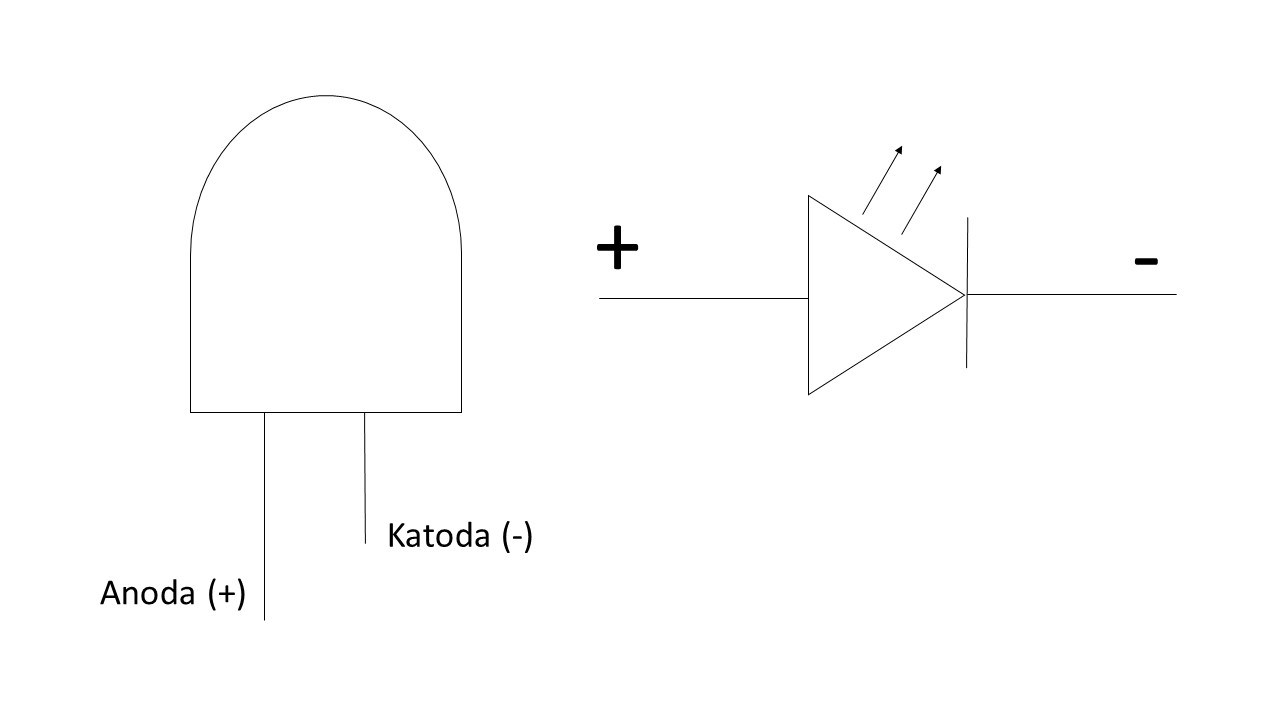
\includegraphics[width=0.6\linewidth]{pics/led}
% 	\caption{\textit{Light emitting diode}.}
% 	\label{fig:led}
% \end{figure}
 
% \section{\textit{Photodetector}}
% \textit{Photodetector} menggunakan fotodioda.....	
% \par


% \section{\textit{Line of Sight}}
% Pada VLC terdapat dua jenis kanal yang terapkan dalam saluran transmisi optik yaitu \textit{Line of Sight} (LOS) dan \textit{Non-Line of Sight} (NLOS)....
% \begin{figure}
% 	\centering
% 	\includegraphics[width=0.4\linewidth]{"pics/TANat/ilustrasi kanal los"}
% 	\caption{Ilustrasi kanal LOS.}
% 	\label{fig:ilustrasi-kanal-los}
% \end{figure}
% Model kanal LOS direpresentasikan pada Gambar \ref{fig:ilustrasi-kanal-los}. Simbol h adalah tinggi \textit{transmitter}, d adalah jarak antara \textit{transmitter} dan \textit{receiver}, dan $\phi$ adalah sudut yang dibentuk antara \textit{transmitter} dan \textit{receiver}.
% \par
% Distribusi sudut dari pola intensitas radiasi dimodelkan menggunakan intensitas lambertian umum yang dinyatakan dengan
% \begin{equation}
% \label {lambertian}
% m=\frac{-\ln 2}{\ln \left(\cos \Phi _{1/2}\right)},
% \end{equation}
% dengan $m$ adalah persamaan lambertian dan $\phi_{1/2}$ adalah nilai \textit{full width at half maximum}.

% Pengiriman data dari \textit{transmitter} ke \textit{receiver} menggunakan kanal \textit{indoor} LOS pada \textit{Optical Wireless Communication} (OWC) yang dapat dirumuskan sebagai berikut \cite{ghassemlooy2013indoor}
% \begin{equation}
% \label{kanal}
% H=\frac{\left(m+1\right)\cdot A_{det}\cdot \cos ^{\left(m+1\right)}\left(\Phi \right)}{2\cdot \pi \cdot d^2},
% \end{equation}
% dengan $A_{det}$ yaitu area \textit{photodetector} di sisi penerima, $d$ merupakan jarak penerima terhadap sisi pengirim, dan $\Phi$ adalah sudut perpindahan terhadap \textit{transmitter}.

% Bab 3 : Perancangan
%-----------------------------------------------------------------------------%
\chapter{\babTiga}
Pada bab ini berisi diagram alir penelitian yang dilakukan dan perancangan simulasi....
%\begin{center}
%	\textbf{BAB III}
%	\par \textbf{PERENCANAAN SISTEM}
%\end{center}
%-----------------------------------------------------------------------------%
% \section{Diagram Alir Penelitian}

% %\begin{flushleft}
% %	\textbf{3.1 Diagram alir penelitian}
% %\end{flushleft}
% %\vspace{-0.5 cm}
% \begin{figure}
% 	\centering
% 	\includegraphics[width=0.9\linewidth]{"pics/TANat/diagram alir baru2"}
% 	\caption{Diagram alir simulasi.}
% 	\label{fig:diagram-alir-baru}
% \end{figure}


% \vspace{-0.5 cm}
% \section{Parameter Input}
% Perancangan simulasi sistem VLC menggunakan beberapa parameter input yang akan digunakan dalam perhitungan. Berikut parameter input pada perhitungan seperti Tabel 3.1.
% \par
% \begin{table}[h]
% 	\centering
% 	\caption{Parameter input sistem.}
% 	\begin{tabular}{|l|l|l|l|}
% 		\hline
% 		\rowcolor[HTML]{E7E6E6} 
% 		No.                  & \multicolumn{2}{l|}{\cellcolor[HTML]{E7E6E6}Parameter}       & Spesifikasi                                                                     \\ \hline
% 		1.                   & \multicolumn{2}{l|}{Ukuran Ruangan}                          & 5x5x3 $m^2$                                                      \\ \hline
% 		&                                        & Jenis               & LED                                                                             \\ \cline{3-4} 
% 		&                                        & Jumlah              & 3                                                                               \\ \cline{3-4} 
% 		&                                        & Daya                & 1 Watt                                                                          \\ \cline{3-4} 
% 		&                                        & Variasi Koordinat 1 & \begin{tabular}[c]{@{}l@{}}(0,5, 4,5, 3)\\ (2,5, 0,5, 3)\\ (4,5, 4,5, 3)\end{tabular} \\ \cline{3-4} 
% 		&                                        & Variasi Koordinat 2 & \begin{tabular}[c]{@{}l@{}}(1,5 , 3,5, 3)\\ (2,5, 1,5, 3)\\ (3,5, 3,5, 3)\end{tabular} \\ \cline{3-4} 
% 		&                                        & Variasi Koordinat 3 & \begin{tabular}[c]{@{}l@{}}(2, 2,5, 3)\\ (2,5, 2, 3)\\ (3, 2,5, 3)\end{tabular}       \\ \cline{3-4} 
% 		\multirow{-7}{*}{2.} & \multirow{-7}{*}{\textit{Transmitter}} & FWHM                & $70^\circ$                                                                      \\ \hline
% 		&                                        & Jenis               & \textit{PIN Photodiode}                                                         \\ \cline{3-4} 
% 		&                                        & Jumlah              & 3                                                                               \\ \cline{3-4} 
% 		&                                        & Variasi Koordinat 1 & \begin{tabular}[c]{@{}l@{}}(2, 3, 0)\\ (2,5, 2, 0)\\ (3, 3, 0)\end{tabular}         \\ \cline{3-4} 
% 		&                                        & Variasi Koordinat 2 & \begin{tabular}[c]{@{}l@{}}(1,5, 3,5, 0)\\ (2,5, 1,5, 0)\\ (3,5, 3,5, 0)\end{tabular} \\ \cline{3-4} 
% 		&                                        & Area Detektor       & $10^{-4} \text{m}^2$                                                \\ \cline{3-4} 
% 		\multirow{-6}{*}{3.} & \multirow{-6}{*}{\textit{Receiver}}    & FOV                 & $60^\circ$                                                                      \\ \hline
% 	\end{tabular}
% \end{table}
% \par
% \vspace{15cm}
% \section{Perhitungan}
% Pada subbab ini memaparkan hasil perhitungan untuk mendapatkan hasil dari parameter performansi sistem yang dihasilkan pada proses simulasi...

% Bab 4 : Pengujian
%-----------------------------------------------------------------------------%
\chapter{\babEmpat}
%\begin{center}
%	\textbf{BAB IV}
%	\par \textbf{ANALISIS SIMULASI SISTEM}
%\end{center}
%-----------------------------------------------------------------------------%
Analisis yang didapatkan berdasakan hasil penelitian....

%-----------------------------------------------------------------------------%
%\section{Analisis Hasil Koordinat \textit{Receiver} Terdeteksi}
%Pada setiap simulasi yang dilakukan menggunakan 3 variasi koordinat letak 3 lampu LED. Setiap simulasi memiliki perbedaan pada letak \textit{receiver} yang akan dideteksi oleh sistem VLC dengan menggunakan algoritma TDOA.
% \section{Skenario 1}
% Pada simulasi skenario 1...
% \section{Skenario 2}
% Pada simulasi skenario 2...

% Bab 5 : Kesimpulan dan Saran
%---------------------------------------------------------------
\chapter{\babLima}
%\begin{center}
%	\textbf{BAB IV}
%	\par \textbf{ANALISIS SIMULASI SISTEM}
%\end{center}



\section{Kesimpulan}
Berdasarkan hasil simulasi dan analisis dapat ditarik kesimpulan sebagai berikut....

\section{Saran}
Saran yang dapat diterapkan pada penelitian selanjutnya yang berkaitan dengan topik Tugas Akhir ini sebagai berikut...

%
% Daftar Pustaka
\renewcommand\bibname{DAFTAR PUSTAKA}
\bibliographystyle{IEEEtran}
\bibliography{ref}
%\includepdf[page=-,pagecommand={},width=\textwidth]{loogbook4}

% Lampiran 
\begin{appendix}
	\pagenumbering{gobble}
	%
% @author  Andreas Febrian
% @version 1.00 
% 
% Hanya sebuah pembatas bertuliskan LAMPIRAN ditengah halaman. 
% 

\begin{titlepage}
	\centering 
	\vspace*{6cm}
	\noindent \Huge{LAMPIRAN}
	\addChapter{LAMPIRAN}
\end{titlepage}


%%	\setcounter{page}{2}
\end{appendix}

\end{document}